\documentclass[border=3pt,tikz]{standalone}
\usepackage{amsmath}
\usetikzlibrary{calc}
\usetikzlibrary{arrows.meta} % for arrow size
\begin{document}
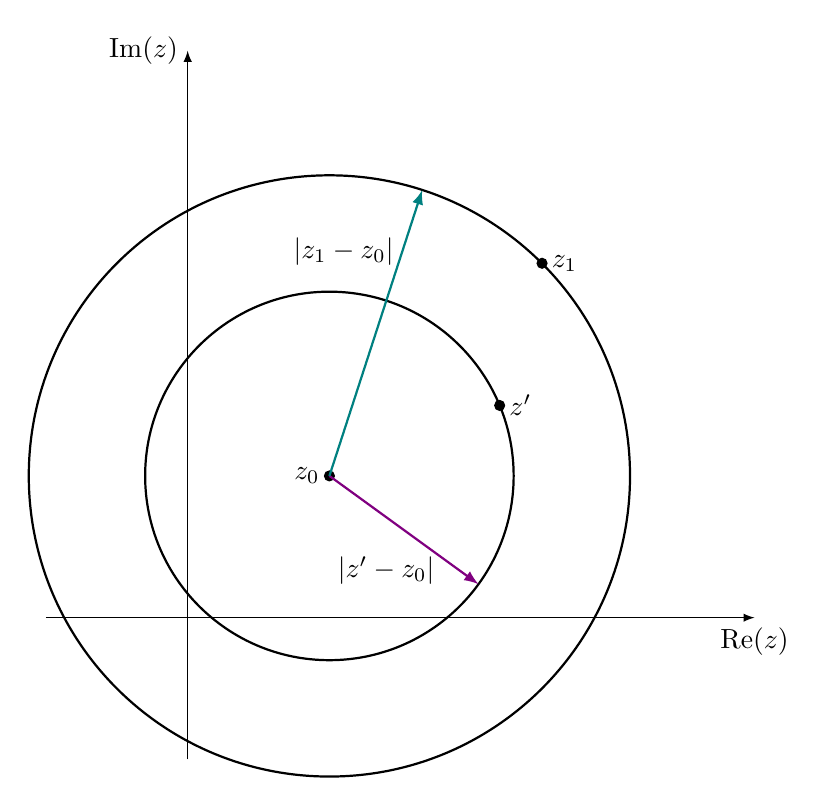
\begin{tikzpicture}[scale=1.8]
    \usetikzlibrary {arrows.meta}
    \usetikzlibrary {calc}
    
    \coordinate (z0) at (1, 1.0);
    \coordinate (z1) at (2.5, 2.5);
    \coordinate (zp) at (2.201, 1.497);
    \draw [-latex] (-1, 0) -- (4, 0) node[below] {Re$(z)$};
    \draw [-latex] (0, -1) -- (0, 4) node[left] {Im$(z)$};
    
    \filldraw [] (z0) circle (1pt) node [left] {$z_0$} ;
    \filldraw [] (z1) circle (1pt) node [right] {$z_1$};
    \filldraw [] (zp) circle (1pt) node [right] {$z^\prime$};
    \draw [thick] (1, 1.0) circle (1.3) ;
    \draw [thick] (1, 1.0) circle (2.121) ;
    
    \draw[violet, thick, -latex] (z0) -- (2.052, 0.236);
    \draw[teal, thick, -latex] (z0) -- (1.655, 3.017);
    
    \node[below] at (1.4, 0.5) {$|z^\prime-z_0|$};
    \node[below] at (1.1, 2.75) {$|z_1-z_0|$};
    \end{tikzpicture}    
\end{document}